\section{$P_1$: Unconstrained Schedule \label{sec:unconstrainedSchedule}}

This section describes a program that finds a charge schedule where buses are allowed to charge without regard to the number of available chargers. This solution is considered ``optimal'' and will be used in later sections to formulate a feasible solution that accounts for the actual number of chargers available.

\begin{table*}
\centering
\caption{Description of the billing structure}
\begin{tabular}{c | c c c}
		                   & On-Peak                & Off-Peak               & Facilities (Both)\\ \hline
		Energy Rate        & \$ 0.058282  /kWh & \$ 0.029624 /kWh  & None \\
		Energy Rate Symbol & $\mu_{\text{e-on}}$    & $\mu_{\text{e-off}}$   & None \\ \hline
		Power Rate  & \$ 15.73 /kW           & None                   & \$ 4.81 /kW \\
		Power Rate Symbol  & $\mu_{\text{p-on}}$    & None            & $\mu_{\text{p-all}}$
	\end{tabular}
	\label{tab:charges} 
\end{table*}


\begin{figure*}
\centering
\scalebox{0.8}{
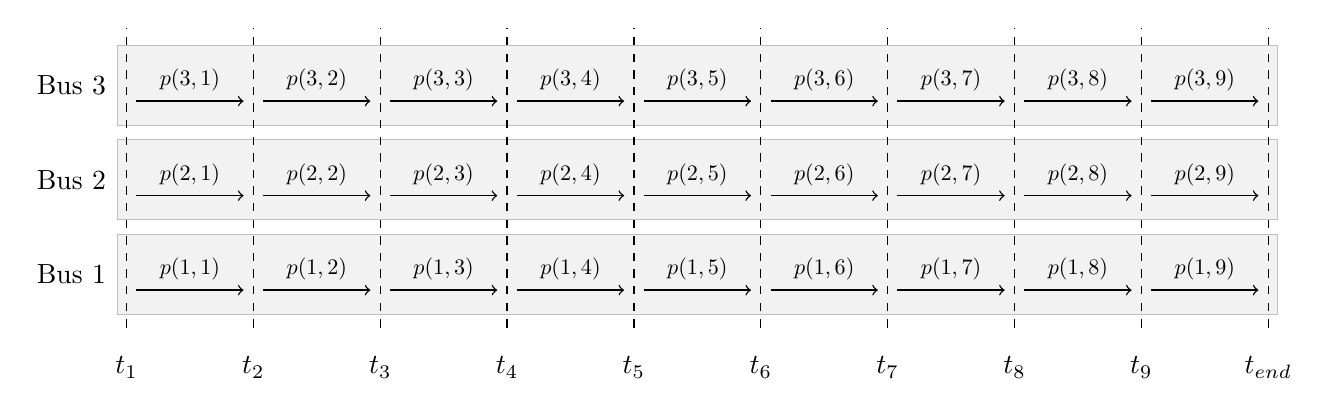
\begin{tikzpicture}
	\node[rectangle, draw=gray!50, fill=gray!10, minimum width=5.8in, minimum height=0.4in](bus1Box) at (7.75,0.8){};
	\node(bus1BoxLabel) at (-0.2, 0.8){Bus 1}; 
	
	\node[rectangle, draw=gray!50, fill=gray!10, minimum width=5.8in, minimum height=0.4in](bus2Box) at (7.75,2){};
	\node(bus1BoxLabel) at (-0.2, 2.0){Bus 2};
	
	\node[rectangle, draw=gray!50, fill=gray!10, minimum width=5.8in, minimum height=0.4in](bus3Box) at (7.75,3.2){};
	\node(bus1BoxLabel) at (-0.2, 3.2){Bus 3};
	
	\foreach \curLab/\preLab[count=\c, evaluate=\c as \pos using {0.5 + (\c - 1)*14.5/9}] in {t_1/t_1, t_2/t_1, t_3/t_2, t_4/t_3, t_5/t_4, t_6/t_7, t_7/t_6, t_8/t_7, t_9/t_8, t_{end}/t_9}
	{
		\node[label=below:$\curLab$](b\c) at (\pos, 0){};
		\node(t) at (\pos, 3.8){};
		\draw[dashed, line width=0.5pt] (b\c.north) -- (t.north); 
		\ifnum\c>1 
			\node(b1Curr) at (\pos, 0.8 - 0.2){};
			\node(b2Curr) at (\pos, 2.0 - 0.2){};
			\node(b3Curr) at (\pos, 3.2 - 0.2){};
			\def\temp{\number\numexpr\c - 1}
			\draw[->, line width=0.5pt] (b1Prev.east) -- node[midway, above]{\scalebox{0.8}{$p(1,\temp)$}}(b1Curr.west);
			\draw[->, line width=0.5pt] (b2Prev.east) -- node[midway, above]{\scalebox{0.8}{$p(2,\temp)$}}(b2Curr.west);
			\draw[->, line width=0.5pt] (b3Prev.east) -- node[midway, above]{\scalebox{0.8}{$p(3,\temp)$}}(b3Curr.west);	
		\fi
			\node(b1Prev) at (\pos, 0.8 - 0.2){};
			\node(b2Prev) at (\pos, 2.0 - 0.2){};
			\node(b3Prev) at (\pos, 3.2 - 0.2){};	
	}
	\path (b9.south) -- node[midway, below=0.1in]{$\hdots$}(b10.south);

\end{tikzpicture}}
\caption{Demonstrates how bus power use is conceptualized}
\label{fig:busPower}
\end{figure*}


\begin{figure*}
\centering
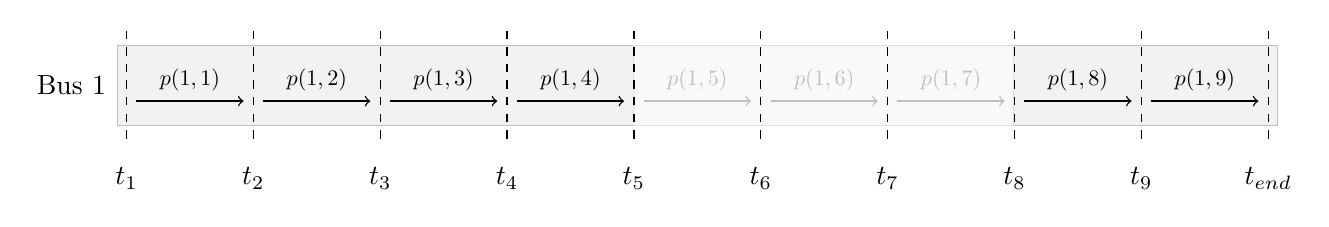
\begin{tikzpicture}
	\node[rectangle, draw=gray!50, fill=gray!10, minimum width=5.8in, minimum height=0.4in](bus1Box) at (7.75,0.8){};
	\node(bus1BoxLabel) at (-0.2, 0.8){Bus 1}; 
	\node[rectangle, draw=gray!25, fill=gray!5, minimum width=1.9in, minimum height=0.4in](bus1Box) at (7.75 + 1.6,0.8){};
	
	\foreach \curLab/\preLab[count=\c, evaluate=\c as \pos using {0.5 + (\c - 1)*14.5/9}] in {t_1/t_1, t_2/t_1, t_3/t_2, t_4/t_3, t_5/t_4, t_6/t_5, t_7/t_6, t_8/t_7, t_9/t_8, t_{end}/t_9}
	{
		\node[label=below:$\curLab$](b\c) at (\pos, 0){};
		\node(t) at (\pos, 1.4){};
		\ifnum\c>1 
			\node(b1Curr) at (\pos, 0.8 - 0.2){};
				\ifnum\c > 5
					\ifnum\c < 9 
						\def\clr{black!25}
					\else
						\def\clr{black}
					\fi
				\else
					\def\clr{black}
				\fi
				\draw[->, line width=0.5pt, \clr] (b1Prev.east) -- node[midway, above]{\scalebox{0.8}{$p(1,\number\numexpr\c-1)$}}(b1Curr.west); 
		\fi
		\node(b1Prev) at (\pos, 0.8 - 0.2){};
		\draw[dashed, line width=0.5pt] (b\c.north) -- (t.north); 
	}
	\path (b9.south) -- node[midway, below=0.1in]{$\hdots$}(b10.south);

\end{tikzpicture}
\caption{Bus schedule with availability}
\label{fig:busAvail}
\end{figure*}



\subsection{Formulation \label{sec:formulation}}

The cost objective we minimize is based on the rate schedule from \cite{rocky_mountain_power_rocky_2021}, which contains two primary elements: the cost of energy and power demand. Energy is billed per kWh using different rates for on-peak and off-peak hours.
%The on-peak rate is more expensive because there is generally more demand for power during this time, whereas off-peak hours tend to be less expensive.
Demand is divided into two components.  The first is a facilities charge which is billed per kW for the highest 15-minute average power use over the course of the month. The second is a demand charge, which is also billed per kW, but is only billed for the highest 15-minute average power usesd during on-peak hours. The rates for each component are given in Table~\ref{tab:charges}.  

Before computing the total monthly cost of electricity, we must define expressions for the average power and energy over time.  Let each day be divided into time intervals of length $\Delta T$ where the average power consumed by bus $i$ during time $j$ is denoted $p(i,j)$ as shown in Fig.~\ref{fig:busPower}. Note that $\Delta T$ may be chosen to be on the order of a second or minute, and expressions for 15-minute averages will be derived later. The solution will yield the average power consumed by each bus during each time interval.

\par The time windows when each bus is available for charging must be accounted for as constraints.  The maximum average power is set to zero when a bus is away from the station. For example, if bus 1 were out on route for times $t_5, t_6,$ and $t_7$, then the average power for those periods would be equal to zero as shown in Fig.~\ref{fig:busAvail}. Let $\bm{b}_{p(i,j)}$ be the average power used by bus $i$ at time index $j$, and $\bm{b}$ be a vector which contains $b_{p(i,j)}$ for each bus and time index. Also let $\mathcal{A} \subset {i\times j}$  be the set of all indices where bus $i$ is in the station during time $t_j$ and let $\tilde{\mathcal{A}}$ be its complement. Also let $p_{\text{max}}$ be the maximum power that a charger can deliver. 
\par The set of constraints that buses do not use power when not in the station are given by
\begin{gather}\label{eqn:obj:power2}
	b_{p(i,j)} = 0 \ \forall i,j \in \tilde{\mathcal{A}}  \\
	0 \leq b_{p(i,j)} \leq p_{\text{max}} \ \forall i,j \in \mathcal{A}
\end{gather}

